%%%%%%%%%%%%%%%%%%%%%%%%%%  ltexpprt.tex  %%%%%%%%%%%%%%%%%%%%%%%%%%%%%%%%
%
% This is ltexpprt.tex, an example file for use with the SIAM LaTeX2E
% Preprint Series macros. It is designed to provide double-column output. 
% Please take the time to read the following comments, as they document
% how to use these macros. This file can be composed and printed out for
% use as sample output.

% Any comments or questions regarding these macros should be directed to:
%
%                 Donna Witzleben
%                 SIAM
%                 3600 University City Science Center
%                 Philadelphia, PA 19104-2688
%                 USA
%                 Telephone: (215) 382-9800
%                 Fax: (215) 386-7999
%                 e-mail: witzleben@siam.org


% This file is to be used as an example for style only. It should not be read
% for content.

%%%%%%%%%%%%%%% PLEASE NOTE THE FOLLOWING STYLE RESTRICTIONS %%%%%%%%%%%%%%%

%%  1. There are no new tags.  Existing LaTeX tags have been formatted to match
%%     the Preprint series style.    
%%
%%  2. You must use \cite in the text to mark your reference citations and 
%%     \bibitem in the listing of references at the end of your chapter. See
%%     the examples in the following file. If you are using BibTeX, please
%%     supply the bst file with the manuscript file.
%% 
%%  3. This macro is set up for two levels of headings (\section and 
%%     \subsection). The macro will automatically number the headings for you.
%%
%%  5. No running heads are to be used for this volume.
%% 
%%  6. Theorems, Lemmas, Definitions, etc. are to be double numbered, 
%%     indicating the section and the occurence of that element
%%     within that section. (For example, the first theorem in the second
%%     section would be numbered 2.1. The macro will 
%%     automatically do the numbering for you.
%%
%%  7. Figures, equations, and tables must be single-numbered. 
%%     Use existing LaTeX tags for these elements.
%%     Numbering will be done automatically.
%%   
%%
%%%%%%%%%%%%%%%%%%%%%%%%%%%%%%%%%%%%%%%%%%%%%%%%%%%%%%%%%%%%%%%%%%%%%%%%%%%%%%%



\documentclass[twoside,leqno,twocolumn]{article}  
\usepackage{ltexpprt} 
\usepackage{amsmath}
\usepackage{color}
\usepackage{url}
\usepackage{hyperref}
\usepackage{subfigure}
\usepackage{amssymb}


\usepackage{xr}
\usepackage{graphicx}
\usepackage{epstopdf}
\usepackage{epsfig}
\usepackage{url,graphics}

% -----------------------------------------------------------------------------
\newcommand{\prithwish}[1]{[{\color{magenta}\textit{Prithwish}\textit{: #1}}]}
\newcommand{\pejman}[1]{[{\color{blue}\textit{Pejman}\textit{: #1}}]}
\newcommand{\naren}[1]{[{\color{green}\textit{Naren}\textit{: #1}}]}

\newcommand{\TODO}[2][NA]{{\color{red}[\textbf{TODO:} #2 \\ \textbf{Assignee:} #1]}}

\begin{document}



%\setcounter{chapter}{2} % If you are doing your chapter as chapter one,
%\setcounter{section}{3} % comment these two lines out.

\title{\Large Forecasting a Moving Target: Ensemble Models for ILI Case
Count Predictions.~\footnotemark[4]}
  \author{Prithwish Chakraborty \footnotemark[1] \\ \and
    Pejman Khadivi \footnotemark[1] \\ \and
  Bryan Lewis \footnotemark[2] \\ \and
    Aravindan Mahendiran \footnotemark[1] \\ \and 
    Patrick Butler \footnotemark[1] \\ \and 
    Elaine Nsoesie \footnotemark[3] \\ \and
    Sumiko Mekaru \footnotemark[3] \\ \and
      John Brownstein \footnotemark[3] \\ \and
    Madhav Marathe \footnotemark[2] \\ \and
    Naren Ramakrishnan \footnotemark[1]
  }
\date{}

\maketitle
% Affiliations Macros to handle 10 authors!!
\footnotetext[1]{Dept. of Computer Science, Virginia Tech,  Blacksbutrg, VA 24061}
\footnotetext[2]{Virginia Bioinformatics Institute, Blacksburg, VA 24061}
\footnotetext[3]{HEALTHMAP}
\footnotetext[4]{IARPA OSI}


 
%\pagenumbering{arabic}
%\setcounter{page}{1}%Leave this line commented out.
\begin{abstract}
  \TODO[Prithwish]{figure out the footnote discrepancies.}\\
  \small\baselineskip=9pt
  This is the text of my  abstract.
  Maximum number of words : 300.\\
  Maximum Keywords: 9.\\
\end{abstract}
 
\section{Introduction.}
% mainfile: ../ltexpprt.tex
Surveillance reports published by health organizations are one of the
primary resources for monitoring influenza like illness (ILI) cases and,
for years, have been the primary source of information used by healthcare
officials for policy decisions. However traditional surveillance
reports are published with a considerable delay and thus recent research
has focused on mining social signals from diverse data sources such as
search engine query volume~\cite{ref1, ref2}, and social
media chatter~\cite{ref3, ref4, ref5, ref6, ref7}.


%and weather data \cite{ref9, Shaman_orig_humidity_link, Shaman_humidity_USA}.
%A number of approaches use only one data
%source (such as \cite{ref1} and \cite{ref4}) while some solutions work
%based on multiple data sources (such as \cite{ref3} and \cite{ref10}). 

%Different solutions have been proposed for different purposes. In a
%number of solutions, the aim is to predict the actual number of ILI
%cases in a specific society \cite{ref2}, \cite{ref1}. These methods are mostly 
%based on classical regression algorithms. At the same time, some research
%~\cite{ref3, ref4} has been directed at monitoring the spatio-temporal distribution of ILI cases in
%a way that can be used by healthcare officials for public reaction
%. The dynamic behavior of epidemics in a
%population is also studied in a number of works in order to understand
%the way that disease propagates through people and between cities
%\cite{ref8}, \cite{ref11}.

One of the pioneering works in this 
space is the work of
Ginsberg et al.~\cite{ref2} where the authors 
predicted weekly ILI case counts
by tracking the volume of search engine queries. This work 
inspired significant follow-on work, e.g.,~\cite{ref1}, where Yuan 
et al. used search query data from Baidu (a popular search 
engine in China) to detect influenza outbreaks. 
More real-time ILI detection~\cite{ref4} systems have been proposed 
by modeling Twitter streams.
%with disease statistics to monitor and predict ILI and cancer 
%in USA. This work also focusses on the importance of tracking both spatial and temporal 
%data. A similar work was presented by Sugamaran and Voss~\cite{ref7} to analyze 
%spatio-temporal spread of the West Nile Virus using Twitter Data. 
%Historical news articles have also been used by Ewing et al. in
%\cite{ref8} to study the spread of influenza pandemic. Authors used data
%mining and network analysis methods for this purpose. Topics are modeled
%by using latent Dirichlet allocation. In \cite{ref12}, Eggo et al. use a
%gravity model for propagation of disease between cities. They used
%Bayesian Markov Chain Monte Carlo methods to estimates parameters of
%their model. %This method can be considered as a single data source
%solution that works with real-time Tweeter data. 

Apart from such social media sources,
there has also been considerable research on 
correlating physical indicators such as climate data with influenza outbreaks. 
The primary advantage of such data sources is that the
effects are much more causal and less noisy. 
Shaman et. al.~\cite{ref9, Shaman_orig_humidity_link, Shaman_humidity_USA} 
explored this area in detail and found absolute humidity 
to be a good indicator of influezna outbreaks.

While the above works have made important strides, there are two important areas that
have been relatively less studied. First, 
only a few works have focused on combining mutiple data sources~\cite{ref10, ref3}
to aid in forecasting. In particular, to the best of our knowledge there has been no work
that investigates the combination of social indicators and physical indicators to forecast
ILI incidence. Second, and more improtantly, official estimates as reported by health
organizations (e.g., WHO, PAHO) are often lagged by several weeks and
even when reported are typically revised for several weeks before the case counts are
finalized. Real-time prediction systems must be designed to handle the forecasting of
such a `moving target'. Finally, most existing works have been retrospective and not set in
the context of a formal data mining validation framework. To overcome these deficiences, we
propose a novel approach to ILI case count forecasting. Our contributions are:
\begin{itemize}
  \item Our approach integrates both social indicators and physical indicators and thus
leverages the selective superiorities of both types of feature sets. We systematize such
integration using a novel matrix factorization-based regression approach
using neighborhood embedding, thus helping account for 
non-linear relationships between the surrogates and the official ILI estimates.
  \item We investigate the efficacy of combining diverse different sources at two
levels: data fusion level, and model level, and discuss the relative (de)merits.
  \item We propose different ways of handling uncertainties in the official 
    estimates and factor these uncertainities into our prediction models.
  \item Finally, we present a detailed and prospective analysis of our proposed methods
    by comparing predictions from a near-horizon real time prediction system to 
    official estimates of ILI case counts in 15 countries of Latin America.
\end{itemize}

%The rest of the paper is organized as follows: we touch upon some related works in 
%Section~\ref{sec:related}, followed by a formal problem definition in Section~\ref{sec:problem},
%and description of our regression framework in Section~\ref{sec:methods}. In Section~\ref{sec:ensemble}, 
%we investigate the question of how best to combine multiple sources and present our strategies to 
%handle the variance in official estimates in Section~\ref{sec:moving}. We conclude with detailed 
%experiments in Section~\ref{sec:experiments}, correspoding results in Section~\ref{sec:results} and present
%our conclusions in Section~\ref{sec:conclusions}.
 %In \cite{ref10}
%different data sources are compared based on different factors such as
%reliability and timeliness. Multiple data sources such as news articles,
%social media, and clinical reports are considered in this study. Authors
%also proposed an integrated framework for a health surveillance system
%that works with multiple data sources. 

%In \cite{ref3}, Denecke et al.
%proposed an event-based approach which can be used for early prediction
%of ILI threats \cite{ref3}. In their method (M-Eco) they consider
%multiple resources such as Tweeter, TV reports, online news articles,
%and blogs. M-Eco is a bi-lingual system that works with information in
%English and German and uses clustering to group documents in to
%clusters. These clusters are then interpreted as signals and used for
%event detection. The system is also based on supervised learning methods
%that rely on signal definitions which have been entered by user.


\section{Related Works.}
% mainfile: ../ltexpprt.tex


Surveillance reports published by health organizations is one of the main resources for monitoring Influenza like illness (ILI) cases and for years have been used by healthcare officials for public reactions. However, these surveillance reports are published with a considerable delay and hence, it takes a long time for health threats to become visible to health officials. Therefore, in recent years, various approaches have been proposed in the literature for monitoring and prediction of influenza epidemics based on data mining and network dynamics methods. These approaches work based on different data sources such as search engine query statistics \cite{ref1}\cite{ref2}, social media micro-blogs \cite{ref3}-\cite{ref7}, news articles \cite{ref8}, and weather data \cite{ref9}. A number of approaches use only one data source (such as \cite{ref1} and \cite{ref4}) while some solutions work based on multiple data sources (such as \cite{ref3} and \cite{ref10}). 

Different solutions have been proposed for different purposes. In a number of solutions, the aim is to predict the actual number of ILI cases in a specific society \cite{ref2}, \cite{ref1}. These methods are mostly work based on regression algorithms. In the second category, the main goal is to monitor the spatio-temporal distribution of ILI cases in a way that can be used by healthcare officials for public reaction \cite{ref3}, \cite{ref4}. The dynamic behavior of epidemics in a population is also studied in a number of works in order to understand the way that disease propagates through people and between cities \cite{ref8}, \cite{ref11}.

One of the first prediction methods based on search engine queries was reported in \cite{ref2}. In their approach, Ginsberg et al. build time series based on Google search queries to track weekly ILI counts. In addition to Google search trends, previously published values in CDC ILI reports are used to learn a simple regression model that predicts weekly influenza counts two weeks ahead of CDC ILI surveillance reports. In \cite{ref1}, Yuan et al. usesearch query data of Baidu (a popular search engine in China) for influenza outbreak prediction. In their approach they use real-time search query results for specific keywords as well as official statistics of influenza to build a regression model that can predict influenza case count one or two weeks in advance. In addition to different data sources, this method differs from \cite{ref2} in terms of the used regression model. In \cite{ref2} a logit-linear model is used while \cite{ref1} uses a simple linear regression model.

Relationship between climate data and influenza outbreak has been studied in \cite{ref9}. Existence of seasonal cycles of influenza epidemics in different climate regions have been known for a long time. In \cite{ref9} Tamerius et al. studied this relationship by considering climatic information from 78 globally distributedsites. Through logistic regression they found out that in “cold-dry” and “humid-rainy” environments strong correlation exists between influenza epidemics and weather conditions.

Online social media data plays an important role in ILI epidemic prediction. In \cite{ref4}, Lee et al. proposed a real-time surveillance system that uses Tweeter data for monitoring and prediction of influenza and cancer in US. This method can be considered as a single data source solution that works with real-time Tweeter data. In \cite{ref4} different types of analysis are used including spatial, temporal, and textual analysis. The purpose of spatial analysis is to determine the distribution of disease in US while temporal analysis is used for tracking the changes in number of tweets with specific keywords. Furthermore, text mining is used for tracking the popularity of disease types, symptoms, and treatments. Results of these analyses are visualized separately and can be used by healthcare officials. An almost similar approach was reported in \cite{ref7} that usesspatio-temporal analysis of Tweeter data to monitor West Nile Virus.Diversity of words in tweets has been studied in \cite{ref5} and \cite{ref6} . In \cite{ref5}, Kanhabua and Nejdl use clustering methods to determine important topics in Tweeter data. They constructed time series for matched keywords and used Jaccard coefficient to determine temporal diversity of tweets. They have noted that this temporal diversity may be correlated with real-world ILI outbreaks. In \cite{ref6} authors studied the dynamic of changes in tweets related to H1N1 virus.

There are a few works in the literature that address using multiple data sources \cite{ref10}, \cite{ref3}. These works highly depend on social media data as well as other public available resources. In \cite{ref10} different data sources are compared based on different factors such as reliability and timeliness. Multiple data sources such as news articles, social media, and clinical reports are considered in this study. Authors also proposed an integrated framework for a health surveillance system that works with multiple data sources. In \cite{ref3}, Denecke et al. proposed an event-based approach which can be used for early prediction of ILI threats \cite{ref3}. In their method (M-Eco) they consider multiple resources such as Tweeter, TV reports, online news articles, and blogs. M-Eco is a bi-lingual system that works with information in English and German and uses clustering to group documents in to clusters. These clusters are then interpreted as signals and used for event detection. The system is also based on supervised learning methods that rely on signal definitions which have been entered by user.

Dynamics of influenza out breaks have been also studied for historically influenza epidemics. In \cite{ref8} and \cite{ref12}, epidemics of 1918 have been studied to understand the behavior of an influenza epidemic in a society. Historical news articles have been used by Ewing et al. in \cite{ref8} to study the spread of influenza pandemic. Authors used data mining and network analysis methods for this purpose. Topics are modeled by using latent Dirichlet allocation. In \cite{ref12}, Eggo et al. use a gravity model for propagation of disease between cities. They used Bayesian Markov Chain Monte Carlo methods to estimates parameters of their model. 

Dynamic behavior of influenza epidemic has been also studied based on synthetic data sources to face with scalability and extensibility problems \cite{ref11}. Network dynamic solutions are used in \cite{ref11} to study the behavior of an epidemic issue in a society. Spread of an infection through a network has been also studied as a general problem in graph-mining \cite{ref13} \cite{ref14}. In \cite{ref14} the main problem is to find the culprits in an epidemic situation based on available data. In \cite{ref13} the main concern is finding the epidemic threshold to distinguish between die-out regimes and break out regimes. 


\section{\label{sec:problem} Problem Formulation.}
% mainfile: ../ltexpprt.tex

\begin{table*}[t!]
  \centering
  \begin{tabular}{|*{2}{l|}}
    \hline
    Abbreviation. & Description \\
    \hline \hline
    ${P}_t$ & Known ILI case count for time point $t$.\\
        $T$ & Max number of time-points for which ILI case count is known.\\
    $\mathcal{X}_t$ & Surroagte data stream at time point $t$ .\\
    $\mathcal{W}_t$ & Weather attributes at time point $t$ .\\
    $\mathcal{T}_t$ & Twitter attributes at time point $t$ .\\
    $\mathcal{H}_t$ & Healthmap attributes at time point $t$ .\\
    $\mathcal{R}_t$ & Reservation data attributes at time point $t$ .\\
    $\mathcal{F}_t$ & Google Search Trends attributes at time point $t$.\\
    ${S}_t$ & Google Flu Trends estimate at time point $t$ .\\
    \hline
  \end{tabular}
  \caption{\label{tb:notations} Notations used in the paper.
  \prithwish{May take this off later and put in the supplemental
section.}}
\end{table*}

In this section, we formally describe the problem.
Let $\mathcal{P} = \langle {P}_1, {P}_2, \dots,
{P}_T \rangle$ denote the known ILI case count for the country under
consideration , where ${P}_t$  denotes the case count for
the time point $t$.
Also let $T$ denote the time-point till which ILI case count is known.
\prithwish{Will have to decide later whether we want to specify PAHO
  here $\rightarrow$ \textnormal{``as reported by the Pan-American Health Organization
(PAHO)~\cite{PAHO:2013}''}}
Corresponding to the ILI case count data, let us denote the available surrogate informations
for the same country by $\mathcal{X} = \langle \mathcal{X}_1, \mathcal{X}_2, 
\dots, \mathcal{X}_{T1}\rangle$, where $T1$ is the time-point till which the surrogate
information is known and $\mathcal{X}_{t}$ denotes the surrogate attributes for time
point $t$. Then we want to find a predictive model ($f$)  for the case count dataas given in  
equation~\ref{eq:problem}.
\begin{equation}
  \label{eq:problem}
  f: \mathcal{P}_t = f\left(\mathcal{P}, \mathcal{X}\right)
\end{equation}



 
\section{\label{sec:methods} Methods.}
% mainfile: ../ltexpprt.tex
%\prithwish{Resolve conflicts for \\
%1. ``time point'' vs ``time point''\\
%2. ``langle'' vs ``left(''}

We employ non-linear temporal regressions over the surrogate attributes to forecast the
case count using three broad models:
\begin{itemize}
  \item Matrix Factorizaiton Based Regression (MF).
  \item Nearest Neighbor Based Regression (NN).
  \item Matrix Factorization Regression using Nearest Neighbor embedding (MFN).
\end{itemize}
For each of the methods, we define two parameters: $\beta$ and $\alpha$. 
$\alpha$ is the {\it lookahead window length}, denoting distance of the time point for prediction from $T$;
$\beta$ is the {\it lookback window length} denoting the number of time points to look back
in order to find the regression relation between the case count and the surrogate data.

We define regression vectors $V_t$  and 
labels $L_t$ for all time points $t, \forall t = 1,\dots, T$
as given in equation~\ref{eq:regressionvector}.
%\prithwish{Check this}
\begin{equation}
  \label{eq:regressionvector}
  \begin{array}{lcl}
    V_t & \equiv & \langle P_{t-\beta - \alpha}, \mathcal{X}_{t-\beta - \alpha}, P_{t + 1 -\beta-\alpha}, \mathcal{X}_{t + 1 - \beta-\alpha}, \dots, \\
        &        & P_{t-\alpha},\mathcal{X}_{t-\alpha} \rangle \\
    L_t & \equiv & P_{t}\\
  \end{array}
\end{equation}
The regression vector for predicting the case count at time point $T' (T +
\alpha > T' > T)$ is given by equation~\ref{eq:regressiontestvector}.
\begin{equation}
  \label{eq:regressiontestvector}
  \begin{array}{lcl}
    V_{T'} & \equiv & \langle P_{T'-\beta - \alpha}, \mathcal{X}_{T'-\beta - \alpha}, P_{t + 1 -\beta-\alpha}, \mathcal{X}_{t + 1 - \beta-\alpha}, \dots, \\
           &        & P_{T'-\alpha},\mathcal{X}_{T'-\alpha} \rangle \\
  \end{array}
\end{equation}
\noindent
Under these definitions we describe the models as follows:
\subsection{\label{sec:model:matrixfactor} Matrix Factorization Based Regression (MF):}
Matrix Factorization is a well accepted technique in
the recommender systems literature, to predict user 
preferences from incomplete user ratings/informations. Typically~\cite{canny2002factor}
a user-preference matrix is factored into an user-factor and
factor-preference matrix. However, such factorizations are incognizant of any 
temporal continuity. As such to enforce temporal continuity, to predict for the time point 
$T' (T +\alpha > T' > T)$ we use the regression vectors 
and labels as defined in equation~\ref{eq:regressionvector} to define a $m \times n$ {\it prediction
matrix} $\mathcal{M}$, as given in equation~\ref{eq:predictionmatrix}:
\begin{equation}
  \label{eq:predictionmatrix}
\mathcal{M} = \left[\begin{array}{ll}
              V_{\alpha + \beta + 1} & L_{\alpha+\beta + 1} \\
                              \vdots & \vdots \\
                               V_{T} & L_T \\
                               V_{T'} & L_{T'} \\ 
    \end{array}
  \right]
\end{equation}

The prediction matrix is factorized into a $f\times m$ factor-feature matrix $U$ and 
a $f\times n$ factor-prediction matrix as:
\[ \widehat{\mathcal{M}}_{i,j} = b_{u,i} + U^T_i \times F_j\]
Here, $b_{i,j}$ is the baseline estimate given by:
 \begin{equation}
   \label{eq:baseline}
   b_{i,j} = \bar{\mathcal{M}} + b_j 
 \end{equation}
 where $\bar{\mathcal{M}}$ represents the all-element average and $b_j$ represents 
 the column wise deviations from the average and is generally a free-parameter, i.e.,
it is fitted as part of the optimization problem.
$U$ and $F$ matrix are estimated by minimizing the error function:
\begin{equation}
  \begin{array}{ll}
  \label{eq:matrix:fit}
  b_*, F, U  & =  \textrm{argmin} (\sum \limits_{i=1}^{m-1} \left(\mathcal{M}_{i,n}  - \widehat{\mathcal{M}}_{i,n} \right)^2 \\ 
  & + \lambda_1\times(\sum \limits_{j=1}^{n}b_j^2 + \sum \limits_{i=1}^{m-1} || U_i||^2 + \sum \limits_{j=1}^{n} || F_j||^2))
\end{array}
\end{equation}
\noindent
where $\lambda_1$ is a regularization parameter. An important design criteria in
the error function of Eqn~\ref{eq:matrix:fit} is the fact that we only compute the error
between the predicted label values and the actual label values i.e., the $n^{th}$ column of the prediction 
matrix $\mathcal{M}$. The rationale behind this choice is the fact that unlike traditional recommender 
systems we are only concerned with the label column and can sacrifice reconstruction accuracies for other 
columns. 

The lookback window $\beta$, the factor size $f$ and the regularization parameter $\lambda_1$ 
are estimated using cross-validation
and the final prediction for time point $T'$ is given by:
\[\widehat{P}_{T'} = b_{m,n} + U_m^T \times F_{m,n} \]

\subsection{\label{sec:model:nearestneighbor} Nearest Neighbor Based Regression (NN):}
For nearest neighbor models, we define a training set $\Gamma_{NN}
= \lbrace V_t, L_t \rbrace$, where $V_t$ represents the regression attributes
and $L_t$ denote the corresponding labels.
Also, let us define the set 
$\mathcal{N}(i) = \lbrace k : \mbox{$V_k$ is one of the top  K nearest neighbors of $V_{i}$} \rbrace$ 
where $K$ indicates the maximum number of nearest neighbors considered.
The predicted count $\widehat{P}_{T'}$ for the time point $T'$ is given as:
\begin{equation} \label{eq:nearestneighbor:pred}
  \begin{array}{lcl}
    \widehat{P}_{T'} & = & \frac{\sum\limits_{k \in \mathcal{N}(T')} \theta_{k}L_{k,T - \alpha}}
    {\sum\limits_{k=1}^{K} \theta_{k}}\\
  \end{array}
\end{equation}
%and $L_{k,T}$ indicates the label of the $k^{th}$ nearest neighbor to $V_{T'}$ in $\Gamma_{NN}$
%at time point $T$. 
\noindent
Here $\theta_k$ indicates the weight assigned to the $k^{th}$ nearest neighbor.
Typically the inverse Euclidean distances to $V_{T'}$ are chosen as the weights.

\subsection{\label{sec:model:nearestmatrix} Matrix Factorization Based
Regression using Nearest Neighbor Embedding (MFN):}
It has been shown in~\cite{koren2008factor} that matrix factorization using nearest neighbor constraints can
outperform classical matrix factorization approach as well as traditional nearest neighbor approaches towards
recommender systems. Here, we modify the method to suit the temporal nature of our problem in similar ways 
as described in section~\ref{sec:model:matrixfactor}. We again define a similar prediction matrix $\mathcal{M}$ 
(see equation~\ref{eq:predictionmatrix}). Following ~\cite{koren2008factor}, we define the 
matrix decomposition rule as 

\begin{equation}
  \label{eq:model:matrixfactornbr}
  \begin{array}{lcl}
    \widehat{\mathcal{M}}_{i,j} & = &  b_{i,j} + U_i^T\times F_j \\
                                &   & + F_j \times |\mathcal{N}(i)|^{-\frac{1}{2}}\sum_{k \in N(i)} (\mathcal{M}_{i,k} - b_{i,k}) x_k \\
  \end{array}
\end{equation}
\noindent
The key difference between equation~\ref{eq:model:matrixfactornbr} and the one proposed in 
~\cite{koren2008factor} is that we don't have any term for implicit feedback and, further,
only the top $K$ neighbors as found through Euclidean distance are used. 
The model is fitted using Eqn~\ref{eq:matrixnbr:fit} as given below:

\begin{equation}
  \label{eq:matrixnbr:fit}
  \begin{array}{ll}
    b_*, F, U, x_*  = \textrm{argmin} &(\sum \limits_{i=1}^{m-1} \left(\mathcal{M}_{i,n} - \widehat{\mathcal{M}}_{i,n}   \right)^2 \\
                    & + \lambda_2\times(\sum \limits_{j=1}^{n}b_j^2 + \sum \limits_{i=1}^{m-1} || U_i||^2 \\
                    & + \sum \limits_{j=1}^{n} || F_j||^2 + \sum_k ||x_k||^2))
  \end{array}
  \end{equation}



\section{Ensemble Approaches.}
% mainfile: ../ltexpprt.tex
%In the last section, we described different regression strategies to correlate
%a specific source with the ILI case count of a specfic country and predict
%future ILI counts. In practice, we edsire to work with a multitude of data
%sources and there are two broad ways to accomplish this objective:
%
%\begin{enumerate}
%  \item Data level fusion, wherein we build a single regressor from all the different data
%    sources to the ILI case count; or
%  \item Model level fusion, wherein we build one regressor for each data source and 
%    subsequently combine the predictions from the models.
%\end{enumerate}
%
%\noindent
%In this section, we describe these fusion methods. Experimental results with 
%both methods are presented in Section~\ref{sec:results}.

In the last section, we described different strategies to correlate a
specific source with the ILI case count of a specific country and predict
future ILI counts.  In practice, we desire to work with a multitude of
data sources and there are two broad ways to accomplish this objective:
(a) data level fusion, where a single regressor is constructed from different
data sources to the ILI case count, and (b) model level fusion, where we
build one regressor for each data source and subsequently combine the
predictions from the models. In this section, we describe these fusion
methods. Experimental results with both methods are presented in Section
~\ref{sec:results}.

\vspace{-1em}
\subsection{\label{sec:fusion:data} Data level fusion:}
Here we express the feature vector $\mathcal{X}$, as a tuple over all the different data 
sources and then proceed with any one of the regression methods as outlined in Section~\ref{sec:methods}.
For example, while combining Twitter and weather data sources (see Fig.~\ref{fig:ili_data_pipeline}), the 
feature vector $\mathcal{X}$ is given by:
\[\mathcal{X}_t = \langle \mathcal{T}_t, \mathcal{W}_t \rangle
\]
where $T_t$ and $W_t$ denote attributes derived from Twitter and weather, respectively.

\vspace{-1em}
\subsection{\label{sec:fusion:model} Model level fusion:}
In this approach, the models are combined using matrix factorization regression with 
nearest neighbor embedding by comparing the
prediction estimates from each model with the actual estimate (since the ground truth
can change as well) and the average
ILI case count for the month for the particular country (to help organize a baseline).
Let us denote the average ILI case count for a particular calendar 
month $I$ for a given country by:
\[
  %\begin{equation*}
  \mu_I = \sum_{t \in I}P_{t}/{|\lbrace t \in I\rbrace|}
  %\mu_I = {1 \over {|\lbrace t \in I\rbrace|}} \sum_{t \in I}P_{t}
%\end{equation*}
\]
%where $|\mathcal{P}|$ is size of $\mathcal{P}$. 
\noindent
Considering $C$ different sources and hence $C$ different models, 
let us denote the prediction for the $t^{th}$ time point 
from the $c^{th}$ model by ${}_c\widehat{P}_t$.

Using these definitions we can now proceed to describe the fusion 
model. Essentially, the model is similar to the one described in 
Section~\ref{sec:model:nearestmatrix}, where the differences can be
found in 
the way we construct the feature vectors. Similar to Eqn~\ref{eq:predictionmatrix},
we construct a prediction  $m'\times n'$ matrix for fusion given by${}_C\mathcal{M}$ where 
the $t^{th}$ row is represented by equation~\ref{eq:fusion:predictionmatrix}.

\vspace{-1em}
\begin{equation}
  \label{eq:fusion:predictionmatrix}
  {}_C\mathcal{M}_{t} = \left[\begin{array}{llll}
      {}_1\widehat{P}_{t}& \dots & {}_C\widehat{P}_t & P_t 
    \end{array}
  \right]
\end{equation}
Then similar to Eqn~\ref{eq:model:matrixfactornbr}, we 
factor this matrix into latent factors, ${}_C U$, ${}_C F$, ${}_C b_*$ as 
given by Eqn~\ref{eq:fusion:matrixfactornbr}:
%\vspace{-1em}
\begin{equation}
  \label{eq:fusion:matrixfactornbr}
  \begin{array}{l}
    {}_C \widehat{\mathcal{M}}_{i,j} =  \mu_i + {}_C b_{j} + {}_C U_i^T\times {}_C F_j \\
                                \, + {}_C F_j \times |{}_C \mathcal{N}(i)|^{-\frac{1}{2}}
    \sum_{k \in {}_C N(i)} ({}_C\mathcal{M}_{i,k} - \mu_i + {}_C b_{k}) {}_Cx_k \\
  \end{array}
\end{equation}
so that the final prediction for the
$T$th data point is given by
\[\widehat{P}_T = {}_C \widehat{\mathcal{M}}_T,n'.\]
The fitting function is given by equation~\ref{eq:fusion:matrixnbr:fit}:
\begin{equation}
  \small
  \label{eq:fusion:matrixnbr:fit}
  \begin{array}{l}
    {}_C b_*, {}_C F, {}_C U, {}_C x_*  = \textrm{argmin} (\sum \limits_{i=1}^{m'-1} \left({}_C \mathcal{M}_{i,n'} - {}_C \widehat{\mathcal{M}}_{i,n'}   \right)^2 \\
     \, + \lambda_3 (\sum \limits_{j=1}^{n'}{}_C b_j^2 + \sum \limits_{i=1}^{m'-1} ||{}_C U_i||^2 
     + \sum \limits_{j=1}^{n'} ||{}_C F_j||^2 + \sum_k ||{}_C x_k||^2))
  \end{array}
\end{equation}
\noindent
As before the free parameters are estimated through cross-validation.



\section{Forecasting a Moving Target.}
% mainfile: ../ltexpprt.tex

One of the key challenges while creating a prospective ILI case count
predictor is the fact that the official estimates are often 
delayed and furthermore even when published the estimates are revised
over a number of weeks before these are finally stabilized.
For this paper, we concentrate on 15 Latin American countries 
as described in Section~\ref{sec:experiments} and consider the official 
ILI estimates from the Pan American Health Organiation (PAHO)~\cite{PAHO:2013}.
%One of the problems with PAHO count dataset is that PAHO count value of a
%specific week may change over time. In other words, PAHO count values are
%unstable for a period of time after they are published for the first time.
Thus we can categorize PAHO count values downloaded on any week
into three different types: (a) the uknnown
PAHO counts reprenseted  by $\ddot{P}_t$, (b) the known and stable PAHO counts
denoted by $\dot{P}_t$, and (c) the known and unstable PAHO counts denoted by
$\tilde{P}_t$. While we want to predict $\ddot{P}_t$, the uncertainity associated
with $\tilde{P}_t$ introduces errors in the predictions. In this section, 
we study the effects of these ``unstable'' data and propose 
three different models to adjust these unstable
values to more accurate ones.

%In order to study the stability behavior of PAHO data, we start with plotting
%relative error of PAHO count values with respect to the stable values. Relative
%error is defined as follows:

%\begin{equation}
%E_{relative} = \frac{\tilde{P}_i - \dot{P}_i}{\dot{P}_i}
%\end{equation}
Figure~\ref{fig:relerrors}, plots the relative error of the unstable Paho data over
its final estimate as a function of time. While it can be seen that different countries 
have different stability characteristics: 
for some countries, PAHO count values are
stabilized very slowly while for others, they are stabilizing faster, as the number of 
updates for a particular week increases, the values generally stabilize.
Stability behavior of PAHO count values were also found to be dependent on the 
time of the year as shown in Figure~\ref{fig:seasonal_relerrors}.
To plot this curve for Argentina, we categorized any week with less than 100 cases to be a low season,
greater than 300 tobe a high season and the remaining values to be low season (the thresholds
were different for different countries).

% talking about priliminary results
\begin{figure}[h]
  \centering
   \begin{tabular}{cc}
     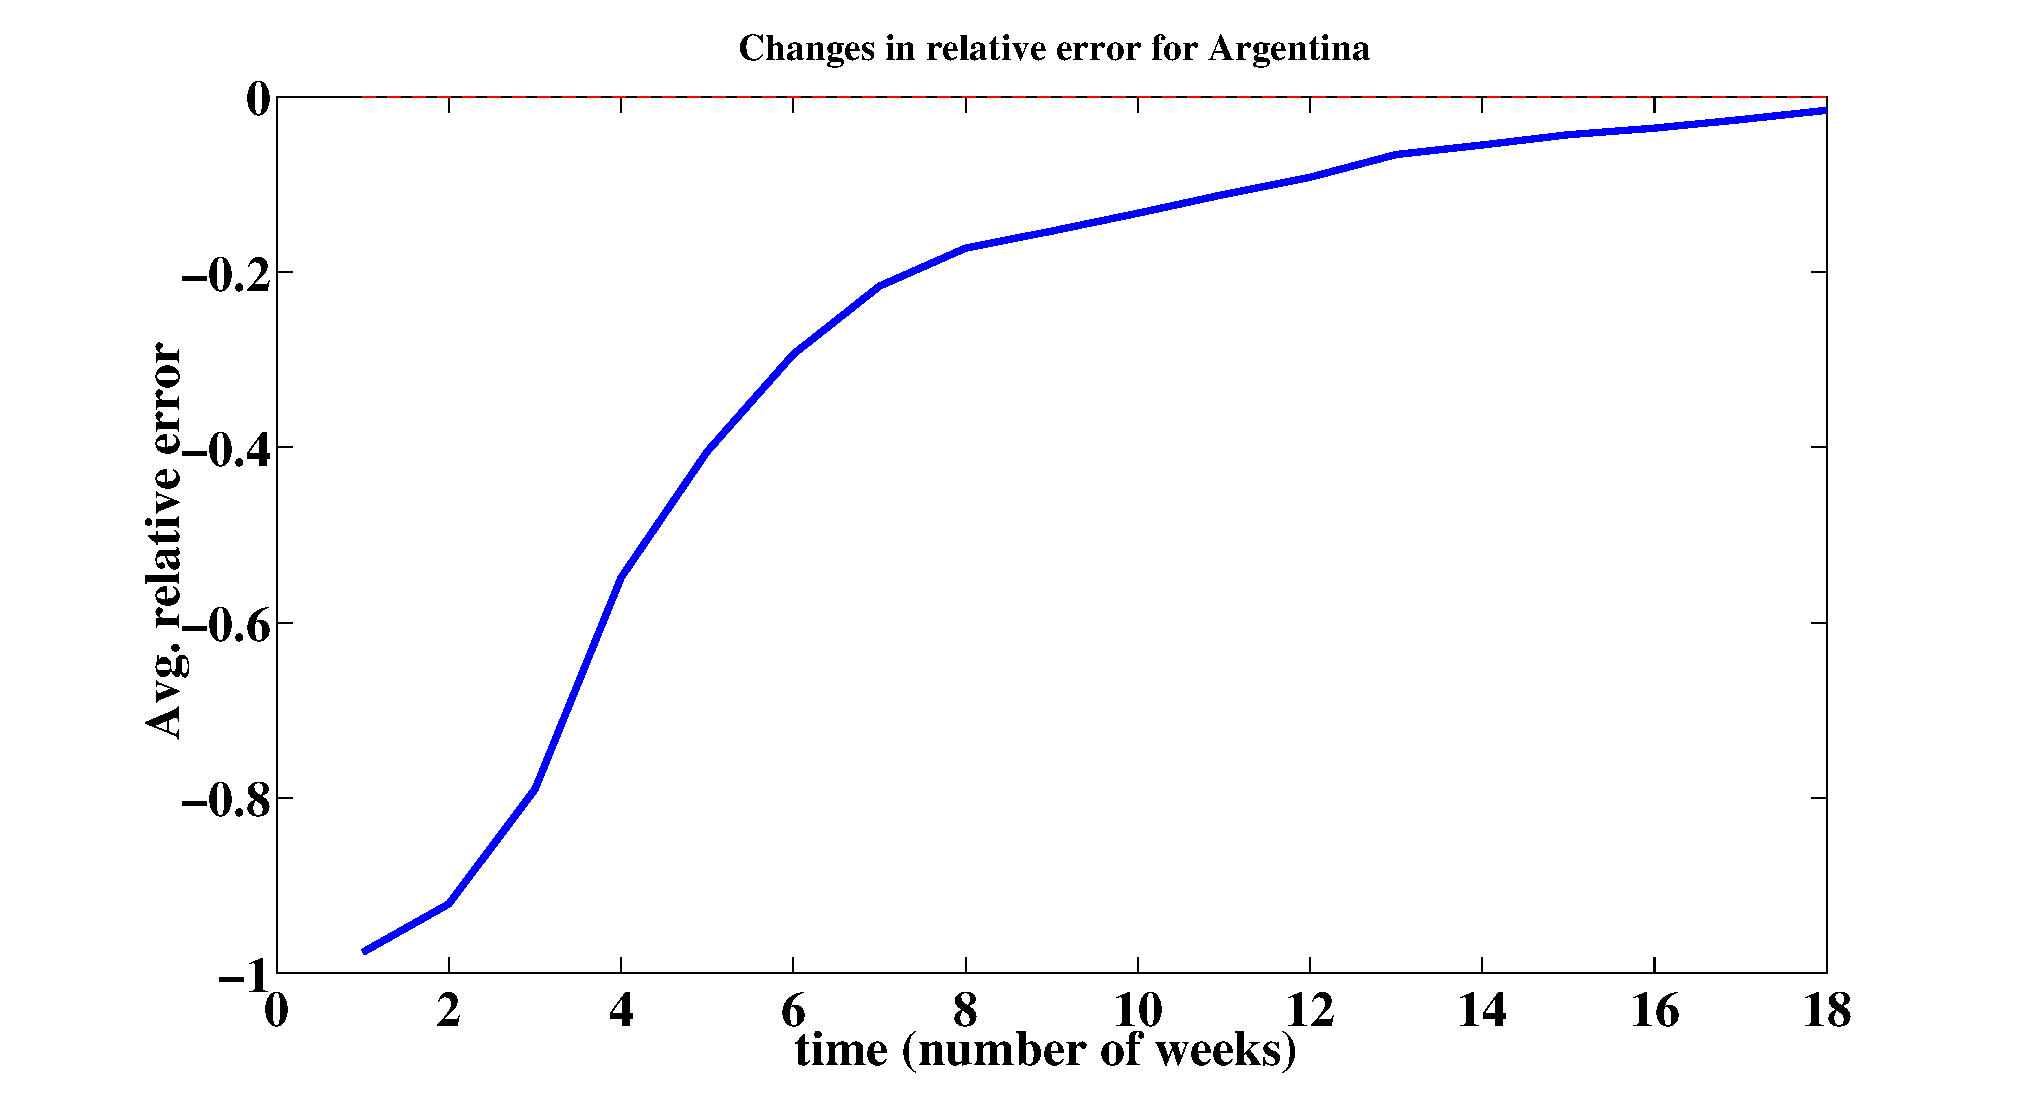
\includegraphics[width=.45\columnwidth]{fig/forpaper_AVGrelativeALLs_Argentina.eps} &
     \includegraphics[width=.45\columnwidth]{fig/forpaper_AVGrelativeALLs_Colombia.eps} \\
 %    \includegraphics[width=.23\textwidth]{forpaper_AVGrelativeALLs_Ecuador.eps} &
 %    \includegraphics[width=.23\textwidth]{forpaper_AVGrelativeALLs_Mexico.eps} \\
      (a) & (b) \\ %& (c) & (d) \\
  \end{tabular}
  \caption{Average relative error of PAHO count values with respect to stable values.
  (a) Argentina,
  (b) and Colombia.
%  (c) Ecuador, and
%  (d) Mexico.
  \label{fig:relerrors}
  }
\end{figure}

\begin{figure}[h]
  \centering
    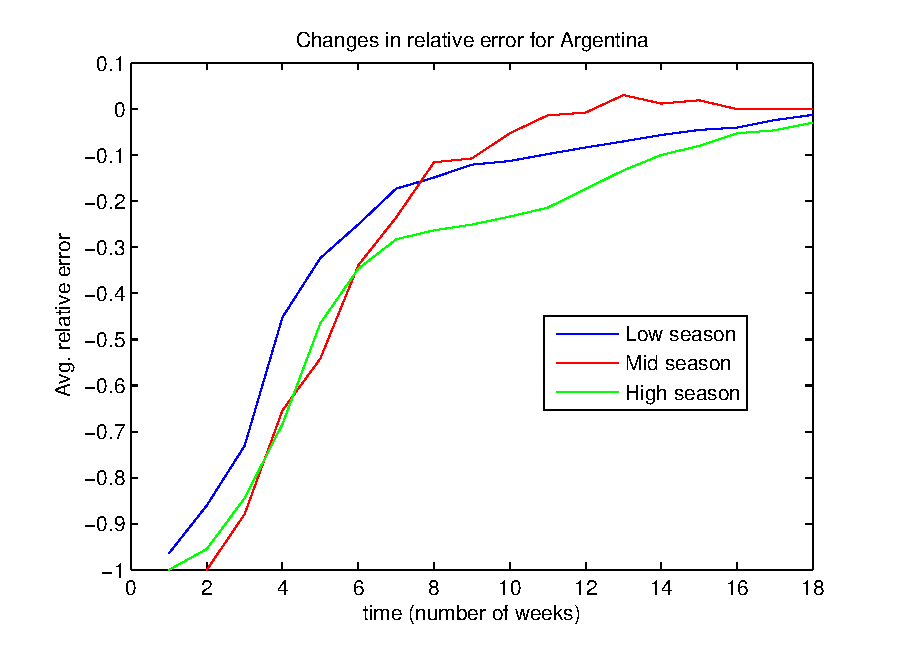
\includegraphics[width=0.5\textwidth]{fig/forpaper_seasonalAVGrelativeALLs_Argentina.eps}
  \caption{Average relative error of PAHO count values for Argentina with respect
  to their stable values for low, mid, and high seasons.}
  \label{fig:seasonal_relerrors}
\end{figure}  

% waiting for publishing stable PAHO values does not work because it is too late

At the same time, the official estimates provide an estimate of number of samples
used to generate the estimate. Preliminary experiments show that
this size is correlated with the accuracy of ILI case counts. In other words,
in general, larger values of statistical population size results in smaller
relative errors for ILI case count.Thus using both the number of samples and the lag in 
uploading the week data, we can use machine learning techniques to revise the officially 
published PAHO estimates. Preliminary results
show that for different seasons and different countries, we have different
stability patterns. Therefore, any PAHO count adjustment method should be
customized for seasons and countries separately. 

Let us assume that $\dot{\mathcal{P}}$ is the set of stable PAHO counts for a
specific country. Also, assume that sequence of updates for each stable PAHO
count value is available. In other words, for $\dot{P}_i$ we have the following
set:
 
\begin{equation}
\dot{\mathcal{P}}_i = \left \{P_i^{(1)},P_i^{(2)},...,P_i^{(m)},...  \right \}
\end{equation}

where, $P_i^{(m)}$ is the value of $P_i$ after $m$ weeks of update. 
For each stable PAHO count value, $\dot{P}_i$, there is a threshold, 
$\dot{T}_i$ that for $m \ge \dot{T}_i$, $P_i^{(m)}$ is stable.

Hence, we have:
\begin{equation}
\dot{\mathcal{P}}_i = \left \{P_i^{(1)},P_i^{(2)},...,P_i
^{(\dot{T}_i-1)},\dot{P}_i,\dot{P}_i,...  \right \}
\end{equation}

In other words, $P_i$ is stabilized after $\dot{T}_i$ weeks.



After recognizing high, low, and mid-season months for the country, we can
categorize each $\dot{P}_i$ to belong to one of these categories. Then, for
category S, an adjustment dataset is constructed named as $\mathcal{P}_A{^S}$
which is defined as follows:

\begin{equation}
\mathcal{P}_A{^S} = \left \{ (1,P_i^{(1)},\dot{P}_i,N_i^{(1)}),...,(m,P_i^{(m)},\dot{P}_i,N_i^{(m)}), ...  \right \}
\end{equation}

Each member of $\mathcal{P}_A{^S}$ is a tuple with four items: first item shows
the time slot that the sample belongs to, second item is the actual unstable
value of $P_i$, third item is the related stable value, and last item,
$N_i^{(m)}$, is the size of statistical population at that week.

In the next step, a linear regression algorithm is used to adjust unstable PAHO
values. In order to adjust value of the PAHO values in the $m$th time slot of
season S, we use $\mathcal{P}_A{^S}$ set to learn $a_0$, $a_1$, $a_2$, and
$a_3$ coefficients in the following equation:

\begin{equation}
\hat{\dot{P}}_i^{(m)} = a_0 + a_1 \times m + a_2 \times P_i^{(m)} + a_3 \times N_i^{(m)}
\label{eq:correctionpaho}
\end{equation}

where, $\hat{\dot{P}}_i^{(m)}$ is the adjusted PAHO count value for the $m$th time slot.

Experimental results show that this adjustment method results in more accurate
known PAHO values. Average relative errors of the published unstable PAHO
values before and after correction for each
country is shown in Figure ~\ref{fig:avgrelerrors}.

%Some experimental results are shown in Figure ~\ref{fig:adjustedrelerrors}.

\begin{figure}[h]
  \centering
    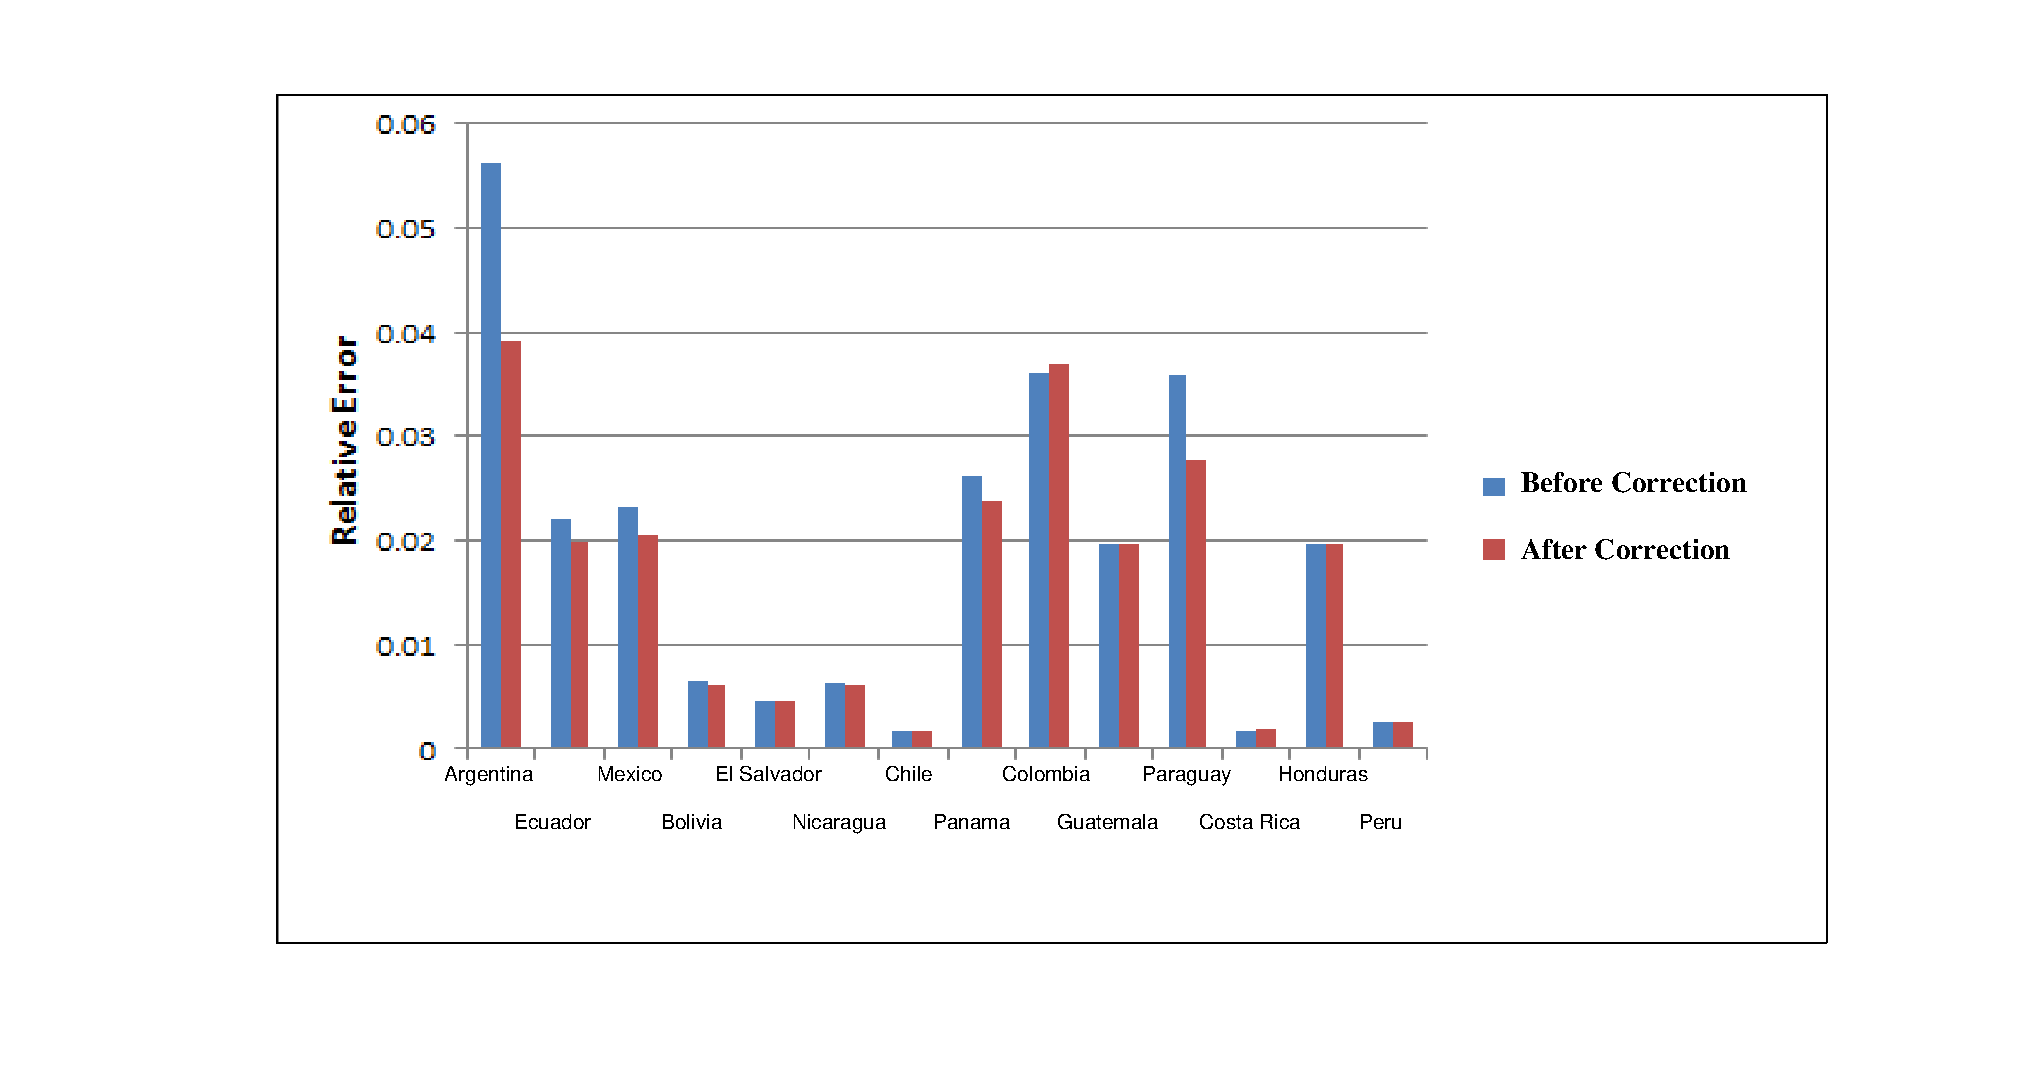
\includegraphics[width=0.5\textwidth]{fig/errs.eps}
  \caption{Average relative error of PAHO count values before and after 
  correction for different countries.}
  \label{fig:avgrelerrors}
\end{figure}

Similar to Eq.~\ref{eq:correctionpaho}, in addition to $P_i^{(m)}$, one can
use only time difference ($m$) or size of population ($N_i^{(m)}$) to correct
unstable PAHO values. Effect of these corrections on overall accuracy of
predictions are shown in Section ~\ref{sec:results}.


\section{Experiments.}
% mainfile: ../ltexpprt.tex

\subsection{Reference Data.}
In this paper, we focus on 15 Latin
American countries viz. Argentina, Bolivia, Costa Rica, Colombia, Chile,
Ecuador,  El Salvador, Guatemala, French Guiana, Honduras, Mexico, Nicaragua,
Paraguay, Panama and Peru. We collected weekly ILI counts
from the official Pan American Health Organization (PAHO)
website~\cite{PAHO:2013}, {\bf every day} from January 2013 to August 2013. The
estimates downloaded every day for each country contain data from January 2010 to the latest
available week on the day of collection. 
%The downloaded data may contain some weeks with no ILI estimates and its next 
%pre-processed to fill the missing using linear interpolation. 
This dataset is stored in a database we refer to as
the {\it Temporal Data Repository} (TDR).  The TDR is also timestamped so that for
any given day, we can readily retrieve the ILI case
counts that were download on that day. This is important as historic data may be updated by
PAHO even a number of weeks after the first update.  For the purpose of experimental validation
we used the data for the period Jan 2010 to December 2012 as the static
training set. We considered Wednesdays of the weeks as a reference day within a week.  For
each Wednesday from Jan 2013 to July 2013, we used the latest available PAHO
data in TDR for that day and predicted 3 weeks from the last available week for
which the PAHO data was available. These predictions are next evaluated against
the final ILI case count as downloaded on September 1, 2013 and we report the
performance of our algorithms in Section~\ref{sec:results}. 

\subsection{Evaluation criteria.}
We evaluate the prediction accuracy of the
different algorithms using a modified version of percentage relative error:

\begin{equation} 
    \label{eq:def:accuracy} 
    \mathcal{A} = \frac{4}{N_p}\sum \limits_{t=t_s}^{t_e}\frac{|P_t -\hat{P}_t| }{max(P_t, \hat{P}_t, 10)}
\end{equation} 
where $t_s$ and $t_e$ indicate the starting and the ending
time point for which predictions were generated.  $N_p$ indicates the number of
time points over the same time period (i.e. $N_p = t_e - t_s + 1$). Note that
the measure is scaled to have values in $[0,4]$ and the denominator is
designed to not over-penalize small deviations from the true ILI case count (e.g., when
the true case count is 0 and the predicted count is 1).
It is to be noted that the accuracy metric so defined is
non-convex and is in general multi-modal. 

%The accuracy criterion was designed according the following criteria:
%\begin{itemize} 
%    \item 
%    The accuracy estimates should reflect the percentage
%    deviation in prediction rather than absolute deviation. 
%     \prithwish{should we justify this?} 
%\item The accuracy estimates must be non-negative.  \item If we
%don't consider the max operator in the denominator, even ``good'' predictions
%such as 1 for an actual count of 0 will be assigned an accuracy score of 0. As
%such we chose a threshold (here 10) for which very small deviations are not
%over-penalized. The threshold was chosen by manually inspecting the span of ILI
%case counts (which were found to lie between 0 and 2000) and subsequent
%feedback from subject experts about the ``interesting'' range of predictions.
%\end{itemize} 


\subsection{Surrogate data sources.} Before
describing our data sources in detail, we describe our overall methodology
for organizing a flu-related disctionary (for tracking in multiple media such
as news, tweets, and search queries).

\subsubsection{\label{sec:keyword} Dictionary creation.} % mainfile: ../ltexpprt.tex

By using multiple methods like pseudo query expansion and correlation analysis using Google Correlate we built a vocabulary of 151 words (both in Spanish and English) that were found to be closely associated with flu. To begin with, our subject matter experts provided us with a set of words that were associated with the flu. These included symptoms, medical synonyms and effects. This set was used as the initial seed for pseudo query expansion, wherein the top 20 web sites returned by Google search for each of these words were crawled. Apart from this, the official CDC website and equivalent websites in each country detailing the causes,symptoms and treatment for influenza was also crawled. Additionally some hand picked websites such as http://www.flufacts.com and http://health.yahoo.net/channel/flu_treatments were also crawled. This entire corpus was then normalized by removing stop words and using porter stemming, post which the words were ranked according to the number of occurrences. The top 500 words for each language was selected. 
Google Correlate is/was a part of Google Trends which allowed users to query the most correlated words in terms of their search volume. Correlate also had a nifty tool wherein one could provide an arbitrary time series and get back a list of words whose search volume was most correlated to the given time series. For our vocabulary building exercise, the ILI case counts published by PAHO on their official website http://ais.paho.org/phip/viz/ed_flu.asp was used to create a time series. For each country, this time series was then fed into Google's Correlate engine and the top 20 correlated words were obtained. These words were a mix of both English and Spanish. As an added exercise, the case count time series was shifted to the left by upto 2 weeks in order to capture the words searched leading up to actual flu infection. Similarly, we shifted the time series to the right to capture the words commonly searched during the tail of the infection. This entire exercise provided us some interesting terms like "ginger" which has been used as a natural herbal remedy in the eastern world. Also, many medications like oseltamivir and tamiflu were found to be highly correlated.   
The set of terms obtained from query expansion and correlation analysis were then pruned by hand to obtain the final vocabulary used by the model. 


We next describe the different data sources.

\subsubsection{Google Flu Trends ($\mathcal{F}$):}
Google Flu Trends~\cite{GFT:2013} (GFT) is a tool based
on~\cite{ginsberg2008detecting} and provided by Google.org which gives weekly
and up-to-date ILI case count estimates using search query volumes. 
Of the countries under
consideration, GFT provides weekly estimates for only 6 of them viz.  Argentina,
Bolivia, Chile, Mexico, Peru and Paraguay. 
These estimates are typically at
a different scale than the ILI case counts provided by PAHO and therefore need
to be scaled accordingly.  We collected this data weekly on Monday from Jan
2013 to Aug 2013. (The data downloaded on a particular day contains the entire
time-series from 2004 to the corresponding week.)
 
\subsubsection{Google Search Trends ($\mathcal{S}$):} Google Search Trends~\cite{GST:2013} is
another tool provided by Google. Using this tool we can download an estimate of
search query volume as a percentage over its own temporal history, filtered
geographically. We download
the search query volume time series for the 114 keywords described earlier
and convert the percentage measures to
absolute values using a static dataset we downloaded on Oct 2012 when Google
Search Trends used to provide absolute query volumes. 

\subsubsection{Twitter ($\mathcal{T}$):} 
Twitter data was collected from Datasift.com
and geotagged using an in-house geocoder. We lemmatized the tweet
contents and used language detection and POS tagging to help differentiate relevant
from irrelevant uses of our keywords 
(e.g., the Spanish word
{\it gripe}, meaning flu, is part of our flu keyword list as opposed to the undesired
and unrelated English word `gripe'). The resulting analysis yields a weekly occurrence
count of our dictionary in tweets.
%Also using the lemmatized versions we
%can match between different parts-of-speech variations of the same word. Using
%the lemma sized equivalents of our keyword dictionary we next parsed the
%enriched Tweets for possible matches with flu related keywords and constructed
%a time series of flu keyword weekly occurrence count. For the country under
%consideration, we denote this time series by 
%$\mathcal{T} = \langle \mathcal{T}_1, \mathcal{T}_2, \dots, \mathcal{T}_{T1} \rangle$.
%
%We started collecting flu filtered Twitter Data from November 2012 and everyday
%we download the corresponding Twitter time-series for each country. As shown in
%Figure~\ref{fig:ili_data_pipeline}, every week we collect 10GB of raw Twitter
%Data which are next enriched to 20GB of structured data. From this dataset, we
%parse flu-related Tweets resulting in around 7GB of data. This data is finally
%abstracted into a multivariate time series over lemmatized versions of the 114
%flu related keywords and added to the TDR. 

\subsubsection{HealthMap ($\mathcal{H}$):} 
Similar to Twitter data, we also collect flu-related
news stories using HealthMap~\cite{HM:2013}, an online global disease alert
system capturing outbreak data from over 50,000 electronic sources [including
expert-curated accounts, such as ProMED-Mail~\cite{chase1996promed}, news media
and official reports from local, national and global public health
organizations.] Using this service we receive flu-related news as a daily feed
which is similarly enriched and filtered to obtain
a multivariate time series over lemmatized version of the keywords. 
While Twitter is more suitable to ascertain general public response, the
HealthMap data provides more detailed information but may capture the trends
at a slower rate. Thus each of these sources offers utility in
capturing different surrogate signals: Twitter offers leading but noisy
indicators whereas HealthMap provides a slightly delayed but more reliable
indicator.

\subsubsection{OpenTable ($\mathcal{O}$):}
We also use data on trends of restaurant table reservations, initially 
studied in~\cite{elaine2013opentable} to be a potential early indicator for
outbreak surveillance, as another surrogate for ILI detection.
This novel data stream is based on the
postulate that a higher than average number of restaurants with table
availabilities in a region can serve as an indicator of an event of interest,
such as increase in flu cases. Table availability was monitored using OpenTable~\cite{Opentable:2013}, 
an online restaurant reservation site with 28,000 restaurants at the time
of this writing. Daily searches were performed starting from September 2012 for
a table for two persons at lunch and dinner; between 12:30-3pm, and between
6-10:30pm. Data was collected for Mexico by city (Cancun, Mexico City, Puebla,
Monterrey, and Guadalajara) and for the entire country. The daily proportion
(proportion used due to changes in the number of restaurants in the system) of
restaurants with available tables was aggregated as a weekly time-series.

%--Since we monitored ten regions at twenty search times, this resulted in 200
%distinct time-series curves.
\begin{figure} 
  \includegraphics[width=3.33in]{fig/humidity_centers.pdf}
  \caption{\label{fig:surveillance} PAHO surveillance centers for the 15 Latin
  American countries.}
\end{figure}

\subsubsection{Weather ($\mathcal{W}$):}
All of the previously described data sources can
be termed as non-physical indicators. These data sources can work as indirect
indicators about the state of the population with respect to flu by exposing
different population characteristics. At the same time, meteorological data can
be considered a more direct and physical driver of influenza transmission~\cite{flu_humidity_physical}. It 
has been shown in~\cite{Shaman_orig_humidity_link, Shaman_humidity_USA, ref9}
that absolute humidity can be directly used to predict the onset of influenza
epidemics. Here, we collected several other meteorological factors such as
temperature and rainfall in addition to humidity from the Global Data
Assimilation System (GDAS) which is a series of weather models run by National
Weather Service's National Centers for Environmental Prediction that provides
detailed meteorological data in near real-time across the globe.  We accessed
the data via an archive hosted by NASA (\url{http://ladsweb.nascom.nasa.gov/})~\cite{HD:2013}, 
and provided in GRIB format. By specifying the resolution and
the geographical boundaries we can collect the data for the countries under
consideration to a resolution of 1 degrees lat/long interval. However, looking
at all the lat/long for a country can often lead to noisy data. As such we
filtered the downloaded data and parsed the meteorological data only around the
PAHO surveillance centers as shown in Fig.~\ref{fig:surveillance}. We also
aggregate this data using weekly averages and thus obtain a resultant time series
for each country. We collected this data weekly from Jan 2013 to August 2013. 

\subsubsection{Temporal Data Repository}
All of the described data sources were
added to a temporal database, ``Temporal Data Repository'' (TDR). Some of the
data sources such as the Weather Data, Twitter Data, HealthMap Data and
OpenTable data once downloaded doesn't change. Also at the time of download
these datasets are updated till the corresponding day.  Thus to extract the
data available at a certain time point for these data sets we can simply
consider the corresponding truncated time series from the latest data. However,
Statistics like Google Search Trends and the PAHO ILI case counts exhibit
variability in past data. In these cases, the actual time series for these datasets are
stored in TDR with the corresponding timestamps. Thus given any time point,
using TDR we can quickly reference the data available at that point of time and
run our algorithm to simulate a prospective analysis scenario.  The entire data
collection process is depicted pictorially in
Figure~\ref{fig:ili_data_pipeline}.





\section{Discussions.}
% mainfile: ../ltexpprt.tex
\begin{itemize}
  \item Table~\ref{tb:comparison_single} Comapring the three regression methods (one for each source and country). 
  \item Discussion GST vs GFT.
  \item Table~\ref{tb:comparison_ensemble} Which Ensembling method to use.
  \item Table~\ref{tb:Ablation} Ablation tests
  \item Table~\ref{tb:moving} Forecasting moving target (three different methods).
  \item Opentable data (more analysis... make this with only Mexico.. just a single plot may suffice). 
\end{itemize}

\begin{table*}[tb!]
\centering
\caption{\label{tb:comparison_single}  Comparing Prediction accuracy of regression models using individual sources.}
\footnotesize
\begin{tabular}{|*{18}{c|}}
\hline
Model               & Sources       & AR & BO & CL & CR & CO & EC & GF & GT & HN & MX & NI & PA & PY & PE & SV & All\\
\hline \hline
\multirow{5}{*}{MF} & $\mathcal{W}$ &2.78&2.46&2.39&2.14&2.70&2.22&2.12&2.63&2.52&2.73&2.31&2.21&2.49&2.77&2.61&2.47\\ 
                    & $\mathcal{H}$ &2.81&2.31&2.22&1.92&2.43&2.04&2.11&2.57&2.33&2.48&2.39&2.15&2.18&2.47&2.33&2.32\\ 
                    & $\mathcal{T}$ &2.37&2.35&2.18&2.03&2.21&2.12&1.83&2.12&2.29&2.03&1.89&2.06&1.96&2.20&2.21&2.12\\ 
                    & $\mathcal{F}$ &2.34&2.11&2.29& N/A& N/A& N/A& N/A& N/A& N?A&2.71& N/A& N/A&2.31&2.24& N/A&2.33\\ 
                    & $\mathcal{S}$ &2.48&2.21&2.33&2.04&2.31&2.21&1.93&2.03&2.15&2.51&2.42&2.52&2.33&1.93&2.30&2.24 \\ 
\hline
\multirow{5}{*}{NN} & $\mathcal{W}$ &2.92&2.93&2.63&2.52&2.66&2.51&2.71&2.82&2.59&2.62&2.55&2.59&2.61&2.80&2.52&2.66\\ 
                    & $\mathcal{H}$ &2.73&3.10&2.42&2.27&2.83&2.64&2.43&2.25&2.71&2.31&2.61&2.35&2.43&2.39&2.52&2.53\\ 
                    & $\mathcal{T}$ &2.72&2.86&2.31&2.62&2.77&2.52&2.71&2.66&2.51&2.44&2.13&2.01&1.77&2.51&2.20&2.45\\ 
                    & $\mathcal{F}$ &2.11&2.21&2.33& N/A& N/A& N/A& N/A& N/A& N?A&2.19& N/A& N/A&2.41&2.32& N/A&2.26\\ 
                    & $\mathcal{S}$ &2.51&2.31&2.41&1.81&2.52&2.41&2.12&2.29&2.51&2.13&2.61&2.14&2.51&1.87&2.12&2.28 \\ 
\hline
\multirow{5}{*}{MFN}& $\mathcal{W}$ &2.99&3.01&2.88&2.53&2.78&2.81&2.77&2.83&2.61&2.70&2.56&2.66&2.82&2.79&2.51&2.75\\ 
                    & $\mathcal{H}$ &2.81&3.13&2.63&2.58&2.91&2.77&2.57&2.63&2.73&2.50&2.61&2.54&2.51&2.69&2.61&2.68\\ 
                    & $\mathcal{T}$ &2.74&3.03&2.51&2.64&2.83&2.51&2.81&2.71&2.60&2.48&2.13&2.55&2.19&2.57&2.31&2.57\\ 
                    & $\mathcal{F}$ &2.33&2.41&2.34& N/A& N/A& N/A& N/A& N/A& N?A&2.69& N/A& N/A&2.54&2.48& N/A&2.46\\ 
                    & $\mathcal{S}$ &2.61&2.44&2.55&2.22&2.61&2.52&2.71&2.31&2.62&2.48&2.61&2.31&2.53&2.23&2.13&2.46\\ 
\hline
\end{tabular}
\end{table*}


\begin{table*}[tb!]
  \centering
  \caption{\label{tb:comparison_ensemble}Comparison of prediction accuracy while combining all data sources
  and using MFN regression.}
  \begin{tabular}{|p{1.5cm}|*{16}{l|}}
\hline
Fusion Level& AR & BO & CL & CR & CO & EC & GF & GT & HN & MX & NI & PA & PY & PE & SV & All\\
\hline \hline
Model       &3.12&3.22&3.03&2.88&2.98&3.13&2.87&2.99&2.87&3.00&2.77&2.82&2.81&2.92&2.87&2.95\\ 
Data        &3.01&2.97&3.13&2.87&2.86&3.04&2.91&2.88&2.72&2.89&2.70&2.60&2.88&2.81&2.92&2.88\\ 
\hline
\end{tabular}
\end{table*}

\begin{table*}[tb!]
  \centering
  \caption{\label{tb:moving} Comparison of prediction accuracy while using model level fusion 
  on MFN regressors and employing PAHO stabilization.}
\begin{tabular}{|p{1.5cm}|*{16}{c|}}
\hline
Correction Method& AR & BO & CL & CR & CO & EC & GF & GT & HN & MX & NI & PA & PY & PE & SV & All\\
\hline \hline
Uncorrected      &3.12&3.22&3.03&2.88&2.98&3.13&2.87&2.99&2.87&3.00&2.77&2.82&2.81&2.92&2.87&2.95\\ 
Weeks Ahead      &3.15&3.24&3.04&2.87&2.97&3.17&2.87&2.99&2.88&3.05&2.77&2.91&3.02&2.91&2.88&2.98\\ 
Num samples      &3.20&3.24&3.03&2.88&2.96&3.12&2.87&3.01&2.89&3.12&2.78&2.92&3.04&2.91&2.87&2.99\\ 
Combined         &3.21&3.24&3.05&2.89&2.96&3.19&2.87&3.00&2.89&3.13&2.77&2.93&3.08&2.92&2.88&3.00\\ 
\hline
\end{tabular}
\end{table*}

\begin{table*}[tb!]
  \centering
  \caption{\label{tb:Ablation} Discovering importance of sources in Model level fusion on MFN 
  regressors by ablating one source at a time.}
\begin{tabular}{|*{17}{c|}}
\hline
Sources & AR & BO & CL & CR & CO & EC & GF & GT & HN & MX & NI & PA & PY & PE & SV & All\\
\hline 
\hline
All               & 3.21& 3.24& 3.05& 2.89& 2.96& 3.19& 2.87& 3.00& 2.89& 3.13& 2.77& 2.93& 3.08& 2.92& 2.88& 3.00\\
w/o $\mathcal{W}$ & 2.91& 2.99& 2.77& 2.71& 2.61& 2.59& 2.66& 2.69& 2.49& 2.78& 2.62& 2.87& 2.60& 2.43& 2.67& 2.69  \\
w/o $\mathcal{H}$ & 3.04& 2.85& 2.89& 2.56& 2.81& 2.77& 2.61& 2.75& 2.75& 2.82& 2.57& 2.75& 2.51& 2.87& 2.71& 2.75  \\
w/o $\mathcal{T}$ & 2.92& 3.14& 2.95& 2.61& 2.72& 2.81& 2.88& 2.79& 2.61& 2.93& 2.74& 2.63& 2.79& 2.74& 2.81& 2.80  \\
w/o $\mathcal{S}$ & 3.19& 3.11& 2.92& 2.64& 2.69& 2.70& 2.89& 2.88& 2.78& 3.07& 2.75& 2.91& 2.80& 2.71& 2.86& 2.86  \\
w/o $\mathcal{F}$ & 3.20& 3.12& 2.88& 2.89& 2.96& 3.19& 2.87& 3.00& 2.83& 3.02& 2.77& 2.93& 2.98& 2.88& 2.88& 2.96  \\
\hline
\end{tabular}
\end{table*}


\begin{table}[tb!]
\centering
\caption{\label{tb:opentable}  ILI case count prediction accruacy for MX using OpenTable Data as a single source and
by combining it with all other sources using Model level fusion.}
\begin{tabular}{|p{1.5cm}|*{2}{l|}p{2cm}|}
\hline
Method& Lunch & Dinner & Lunch and Dinner Time \\
\hline \hline
MF   & 1.92 & 2.23 & 2.31 \\
NN   & 1.99 & 1.83 & 2.11 \\
MFN  & 2.11 & 2.31 & 2.44 \\
Model Fusion & 2.96 & 2.87 & 2.99 \\
\hline
\end{tabular}
\end{table}




\section{Conclusions and Further Work.}
% mainfile: ../ltexpprt.tex
To forecast ILI over a range of Latin American countries, we have
explored a gamut of options pertaining to data sources, fusion
possibilities, and corrections to track a moving target. Our results
demonstrate that there are significant opportunities to improve
forecasting performance and selective superiorities among data sources
that can be leveraged.  Our future work focuses on reconciling the
phenomenological models developed here with true epidemiological models
to that we can develop not just near-term forecasts as done here but
also identify long-range characteristics of the epidemic as it unfolds.
We also aim to explore the inter-country characteristics of ILI
profiles in future.


%FOR NOW. TO be replaced by the bbl
\bibliographystyle{IEEEtran}
\bibliography{references}

%\begin{thebibliography}{99}

%\bibitem{GUIDE}
%R.~E. Bank, {\em PLTMG  users' guide, edition 5.0}, tech. report,
  %Department of Mathematics, University of California, San Diego, CA, 1988.


%\bibitem{LIU}
%J.~W.~H. Liu, {\em A compact row storage scheme for cholesky factors
  %using elimination trees}, ACM TOMS, 12 (1986), pp.~127--148.

%\bibitem{LIU2}
%\sameauthor , {\em The role of
  %elimination trees in sparse factorization}, Tech. Report CS-87-12,Department
  %of Computer Science, York University, Ontario, Canada, 1987.

%\bibitem{ROSE72}
%D.~J. Rose, {\em A graph theoretic study of the numeric solution of
  %sparse positive definite systems}, in Graph Theory and Computing, Academic  Press, New
%York, 1972.


%\end{thebibliography}
\end{document}
